\documentclass[12pt,t]{beamer}
\usepackage{graphicx}
\setbeameroption{hide notes}
\setbeamertemplate{note page}[plain]
\usepackage{listings}

% set up listing environment
\lstset{language=bash,
        basicstyle=\ttfamily\scriptsize,
        frame=single,
        commentstyle=,
        backgroundcolor=\color{darkgray},
        showspaces=false,
        showstringspaces=false
        }

% get rid of junk
\usetheme{default}
\beamertemplatenavigationsymbolsempty
\hypersetup{pdfpagemode=UseNone} % don't show bookmarks on initial view


% font
\usepackage{fontspec}
\setsansfont
  [ ExternalLocation = ../fonts/ ,
    UprightFont = *-regular , 
    BoldFont = *-bold ,
    ItalicFont = *-italic ,
    BoldItalicFont = *-bolditalic ]{texgyreheros}
\setbeamerfont{note page}{family*=pplx,size=\footnotesize} % Palatino for notes
% "TeX Gyre Heros can be used as a replacement for Helvetica"
% I've placed them in ../fonts/; alternatively you can install them
% permanently on your system as follows:
%     Download http://www.gust.org.pl/projects/e-foundry/tex-gyre/heros/qhv2.004otf.zip
%     In Unix, unzip it into ~/.fonts
%     In Mac, unzip it, double-click the .otf files, and install using "FontBook"

% named colors
\definecolor{offwhite}{RGB}{249,242,215}
\definecolor{foreground}{RGB}{255,255,255}
\definecolor{background}{RGB}{24,24,24}
\definecolor{title}{RGB}{107,174,214}
\definecolor{gray}{RGB}{155,155,155}
\definecolor{subtitle}{RGB}{102,255,204}
\definecolor{hilit}{RGB}{102,255,204}
\definecolor{vhilit}{RGB}{255,111,207}
\definecolor{nhilit}{RGB}{128,0,128}  % hilit color in notes
\definecolor{nvhilit}{RGB}{255,0,128} % vhilit for notes
\definecolor{lolit}{RGB}{155,155,155}

\newcommand{\hilit}{\color{hilit}}
\newcommand{\vhilit}{\color{vhilit}}
\newcommand{\nhilit}{\color{nhilit}}
\newcommand{\nvhilit}{\color{nvhilit}}
\newcommand{\lolit}{\color{lolit}}

% use those colors
\setbeamercolor{titlelike}{fg=title}
\setbeamercolor{subtitle}{fg=subtitle}
\setbeamercolor{institute}{fg=gray}
\setbeamercolor{normal text}{fg=foreground,bg=background}
\setbeamercolor{item}{fg=foreground} % color of bullets
\setbeamercolor{subitem}{fg=gray}
\setbeamercolor{itemize/enumerate subbody}{fg=gray}
\setbeamertemplate{itemize subitem}{{\textendash}}
\setbeamerfont{itemize/enumerate subbody}{size=\footnotesize}
\setbeamerfont{itemize/enumerate subitem}{size=\footnotesize}

% page number
\setbeamertemplate{footline}{%
    \raisebox{5pt}{\makebox[\paperwidth]{\hfill\makebox[20pt]{\lolit
          \scriptsize\insertframenumber}}}\hspace*{5pt}}

% add a bit of space at the top of the notes page
\addtobeamertemplate{note page}{\setlength{\parskip}{12pt}}

% default link color
\hypersetup{colorlinks, urlcolor={hilit}}

% a few macros
\newcommand{\bi}{\begin{itemize}}
\newcommand{\bbi}{\vspace{24pt} \begin{itemize} \itemsep8pt}
\newcommand{\ei}{\end{itemize}}
\newcommand{\ig}{\includegraphics}
\newcommand{\subt}[1]{{\footnotesize \color{subtitle} {#1}}}
\newcommand{\ttsm}{\tt \small}
\newcommand{\ttfn}{\tt \footnotesize}
\newcommand{\figh}[2]{\centerline{\includegraphics[height=#2\textheight]{#1}}}
\newcommand{\figw}[2]{\centerline{\includegraphics[width=#2\textwidth]{#1}}}


%%%%%%%%%%%%%%%%%%%%%%%%%%%%%%%%%%%%%%%%%%%%%%%%%%%%%%%%%%%%%%%%%%%%%%
% end of header
%%%%%%%%%%%%%%%%%%%%%%%%%%%%%%%%%%%%%%%%%%%%%%%%%%%%%%%%%%%%%%%%%%%%%%

% title info
\title{Writing reproducible reports}
\subtitle{knitr with R Markdown}
\author{\href{http://kbroman.org}{Karl Broman}}
\institute{Biostatistics \& Medical Informatics, UW{\textendash}Madison}
\date{\href{http://kbroman.org}{\tt \scriptsize \color{foreground} kbroman.org}
\\[-4pt]
\href{https://github.com/kbroman}{\tt \scriptsize \color{foreground} github.com/kbroman}
\\[-4pt]
\href{https://twitter.com/kwbroman}{\tt \scriptsize \color{foreground} @kwbroman}
\\[-4pt]
{\scriptsize Course web: \href{http://kbroman.org/Tools4RR}{\tt kbroman.org/Tools4RR}}
}


\begin{document}

% title slide
{
\setbeamertemplate{footline}{} % no page number here
\frame{
  \titlepage

\note{Statisticians write a lot of reports, describing the results of
  data analyses. It's best if such reports are fully reproducible:
  that the data and code are available, and that there's a clear and
  automatic path from data and code to the final report.

  knitr is ideal for this effort. It's a system for combining code and
  text into a single document. Process the document, and the code is
  replaced with the results and figures that it generates.

  I've found it most efficient to produce informal analysis reports as
  web pages. Markdown is a system for writing simple,
  readable text, with the sort of marks that you might use in an email
  message, that gets converted to nicely formatted html-based web pages.

  My goal in this lecture is to show you how to use knitr with R
  Markdown (a variant of Markdown) to make such
  reproducible reports, and to convince you that this is the way that
  you should be constructing such analysis reports.

  I'd originally planned to also cover knitr with AsciiDoc, but I
  decided to drop it; it's best to focus on Markdown.
}
} }


\begin{frame}[c]{knitr in a knutshell}

\centerline{\Large \href{http://kbroman.org/knitr_knutshell}{\tt kbroman.org/knitr\_knutshell}}

\note{I wrote a short tutorial on knitr, covering a bit more than I'll
  cover in this lecture.

  I'd be glad for suggestions, corrections, or questions.
}
\end{frame}






\begin{frame}{Data analysis reports}

\vspace{24pt}

\bi
\itemsep24pt
\item Figures/tables + email
\item Static \LaTeX\ or Word document
\item knitr/Sweave + \LaTeX\ $\rightarrow$ PDF
\item knitr + Markdown $\rightarrow$ Web page
\ei

\note{Statisticians write a lot of reports. You do a bunch of
  analyses, create a bunch of figures and tables, and you want to
  describe what you've done to a collaborator.

  When I was first starting out, I'd create a bunch of figures and
  tables and email them to my collaborator with a description of the
  findings in the body of the email. That was cumbersome for me and
  for the collaborator. (``Which figure are we talking about, again?'')

  I moved towards writing formal reports in
  \LaTeX\ and sending my collaborator a
  PDF. But that was a lot of work, and if I later wanted to re-run
  things (e.g., if additional data were added), it was a real hassle.

  Sweave + \LaTeX\ was a big help, but it's a pain to deal with page
  breaks.

  Web pages, produced with knitr and Markdown, are ideal. You can make
  super-tall multi-panel figures that show the full details, without
  worrying page breaks. And hyperlinks are more convenient, too.
}
\end{frame}


\begin{frame}[c]{}

\centering
What if the data change?

\vspace{36pt}

What if you used the wrong version of the data?

\note{If data are added, will it be easy to go back and re-do your
  analyses, or is there a lot of copying-and-pasting and editing to be
  done?

  I usually start an analysis report with a summary of the experiment,
  scientific questions, and the data. Recently, a collaborator noticed
  that I'd used an old version of the data. (I'd cited sample
  sizes, and so he could see that I didn't have the full set.)

  He said, ``I'm really sorry you did all that work on the incomplete
  dataset.''

  But actually, it didn't take long to find the right file, and the
  revised analysis was derived instantaneously, as I'd used knitr.
}

\end{frame}


\begin{frame}[fragile]{knitr code chunks}

\vspace{6pt}

\href{https://github.com/kbroman/Tools4RR/blob/master/03_KnitrMarkdown/Examples/example1.Rmd}{Input to knitr}:
\begin{lstlisting}
We see that this is an intercross with `r nind(sug)`
individuals. There are `r nphe(sug)` phenotypes, and genotype
data at `r totmar(sug)` markers across the `r nchr(sug)`
autosomes.  The genotype data is quite complete.

```{r summary_plot, fig.height=8}
plot(sug)
```
\end{lstlisting}

\vfill

\href{https://github.com/kbroman/Tools4RR/blob/master/03_KnitrMarkdown/Examples/example1.md}{Output from knitr}:
\begin{lstlisting}
We see that this is an intercross with 163
individuals. There are 6 phenotypes, and genotype
data at 93 markers across the 19
autosomes.  The genotype data is quite complete.

```r
plot(sug)
```

![plot of chunk summary_plot](RmdFigs/summary_plot.png)
\end{lstlisting}


\note{The basic idea in knitr is that your regular text document will
  be interrupted by chunks of code delimited in a special way.

  This example is with R Markdown.

  There are in-line bits of code indicated with backticks.
  When the document is processed by knitr, they'll be evaluated and
  replaced by the result.

  Larger code chunks with three backticks. This one will produce a
  plot. When processed by knitr, an image file will be created and a
  link to the image will be inserted at that location.

  In knitr, different types of text have different ways of delimiting
  code chunks, because it's basically going to do a
  search-and-replace and depending on the form of text, different
  patterns will be easier to find.
}
\end{frame}


\begin{frame}[fragile]{html}

\vspace{6pt}

\begin{lstlisting}
<!DOCTYPE html>
<html lang="em">
<head>
  <meta charset=utf-8"/>
  <title>Example html file</title>
</head>

<body>
<h1>Markdown example</h1>

<p>Use a bit of <strong>bold</strong> or <em>italics</em>. Use
backticks to indicate <code>code</code> that will be rendered
in monospace.</p>

<ul>
<li>This is part of a list</li>
<li>another item</li>
</ul>

</body>
</html>
\end{lstlisting}

\vfill

\hfill {\footnotesize \lolit [\href{http://kbroman.github.io/knitr_knutshell/assets/markdown_example.html}{Example}]}

\note{It's helpful to know a bit of html, which is the markup
language that web pages are written in. html really isn't that hard;
it's just cumbersome.

An html document contains pairs of tags to indicate content, like
{\tt <h1>} and {\tt </h1>} to indicate that the enclosed text is a
``level one header'', or {\tt <em>} and {\tt </em>} to indicate emphasis
(generally italics). A web browser will parse the html tags and
render the web page, often using a cascading style sheet (CSS) to
define the precise style of the different elements.

Note that there are six levels of headers, with tags
{\tt <h1>}, {\tt <h2>}, {\tt <h3>}, \dots, {\tt <h6>}.
Think of these as the title,
section, subsection, sub-subsection, \dots
}
\end{frame}


\begin{frame}[fragile]{CSS}

\vspace{24pt}

\begin{lstlisting}
ul,ol {
  margin: 0 0 0 35px;
}

a {
  color: purple;
  text-decoration: none;
  background-color: transparent;
}

a:hover
{
  color: purple;
  background: #CAFFFF;
}
\end{lstlisting}

\vspace{24pt}

\hfill {\footnotesize \lolit
[\href{http://kevinburke.bitbucket.org/markdowncss/markdown.css}{Example}]}

\note{I don't really want to talk about CSS, but I thought I should at
  least acknowledge its existence.

  CSS is really important for defining how your document will
  appear. Much of the time, you just want to find someone else's CSS
  document that is satisfactory to you.
}
\end{frame}


\begin{frame}[fragile]{Markdown}

\vspace{6pt}

\begin{lstlisting}
# Markdown example

Use a bit of **bold** or _italics_. Use backticks to indicate
`code` that will be rendered in monospace.

- This is part of a list
- another item

Include blocks of code using three backticks:

```
x <- rnorm(100)
```

Or indent four spaces:

    mean(x)
    sd(x)

And it's easy to create links, like to
[Markdown](http://daringfireball.net/projects/markdown/).
\end{lstlisting}

\vfill

\hfill {\footnotesize \lolit
[\href{http://kbroman.github.io/knitr_knutshell/assets/markdown_example.md}{Example} |
\href{https://github.com/adam-p/markdown-here/wiki/Markdown-Cheatsheet}{MD cheat sheet}]}

\note{Markdown is a system for writing simple, readable text that is
  easily converted into html. The reason it's useful to know a bit of
  html is that then you have a better idea how the final product will
  look. (Plus, if you want to get fancy, you can just insert a bit of
  html within the Markdown document.)

  Markdown is just a system of marks that will get searched-and-
  replaced to create an html document. A big advantage of the Markdown
  marks is that the source document is much like what you might write
  in an email, and so it's much more human-readable.

  Github (which we'll talk about next week) automatically renders
  Markdown files as html, and you can use Markdown for ReadMe files.
  And the website for this course is mostly in Markdown.
}
\end{frame}




\begin{frame}[fragile]{R Markdown}

\vspace{24pt}

\bi
\itemsep12pt
\item \href{http://rmarkdown.rstudio.com}{R Markdown} is a variant of Markdown, developed at
  \href{http://www.rstudio.com}{RStudio.com}
\item Markdown + knitr + extras
\item A few extra marks
\item \href{http://www.rstudio.com/ide/docs/authoring/using_markdown_equations}{\LaTeX\ equations}
\item Bundle images into the final html file
\ei

\note{R Markdown is a variant of Markdown developed by the folks at
  RStudio.

  It's Markdown with knitr code chunks, but there are a number of
  added features,  most importantly the ability to use
  \LaTeX\ equations.
}
\end{frame}


\begin{frame}[fragile]{Code chunks, again}

\vspace{6pt}

\begin{lstlisting}
```{r knitr_options, include=FALSE}
knitr::opts_chunk$set(fig.width=12, fig.height=4,
                      fig.path='Figs/', warning=FALSE,
                      message=FALSE)
set.seed(53079239)
```

### Preliminaries

Load the R/qtl package using the `library` function:

```{r load_qtl}
library(qtl)
```

To get help on the read.cross function in R, type the
following:

```{r help, eval=FALSE}
?read.cross
```
\end{lstlisting}

\vfill

\hfill {\footnotesize \lolit
[\href{https://github.com/kbroman/knitr_knutshell/blob/gh-pages/assets/knitr_example.Rmd}{Example}]}


\note{A couple of additional points about code chunks.

You can (and should) assign names to the code chunks. It will make it
easier to fix errors, and figure files will be named based on the
name of the chunk that produces them.

Code chunks can also have options, like {\tt include=FALSE} and {\tt eval=FALSE}.
And you can define global options, which will apply to all subsequent
chunks.
}
\end{frame}


\begin{frame}[fragile]{Chunk options}

\vspace{6pt}

\renewcommand{\arraystretch}{1.3}
\begin{tabular}{ll}
{\tt echo=FALSE}     & \lolit Don't include the code \\
{\tt results="hide"} & \lolit Don't include the output \\
{\tt include=FALSE}  & \lolit Don't show code or output \\
{\tt eval=FALSE}     & \lolit Don't evaluate the code at all \\
{\tt warning=FALSE}  & \lolit Don't show R warnings \\
{\tt message=FALSE}  & \lolit Don't show R messages \\
{\tt fig.width={\lolit \#}}   & \lolit Width of figure \\
{\tt fig.height={\lolit \#}}  & \lolit Height of figure \\
{\tt fig.path="Figs/"} & \lolit Path for figure files \\
\end{tabular}

\vspace{24pt}

There are \href{http://yihui.name/knitr/options#chunk_options}{lots of chunk options}.

\note{These are the chunk options that I use most, but there are lots
  more. Each should be valid R code, and can be basically any valid
  R code, so you can get pretty fancy.

  The ending slash in {\tt fig.path} is important, as this is just pasted to
  the front of the figure file names. If not included, the figures
  would be in the main directory but with names starting with ``{\tt Figs}''.
}
\end{frame}



\begin{frame}[fragile]{Global chunk options}

\vspace{6pt}

\begin{lstlisting}
```{r knitr_options, include=FALSE}
knitr::opts_chunk$set(fig.width=12, fig.height=4,
                      fig.path='Figs/', warning=FALSE,
                      message=FALSE, include=FALSE,
                      echo=FALSE)
set.seed(53079239)
```

```{r make_plot, fig.width=8, include=TRUE}
x <- rnorm(100)
y <- 2*x + rnorm(100)
plot(x, y)
```
\end{lstlisting}

\vfill

\bi
\itemsep12pt
\item Use global chunk options rather than repeat the same options over and over.
\item You can override the global values in specific chunks.
\ei

\note{I'll often use {\tt include=FALSE} and {\tt echo=FALSE} in a report to a
  collaborator, as they won't want to see the code and raw
  results. I'll then use {\tt include=TRUE} for the figure chunks.

  And I'll set some default choice for figure heights and widths but
  then adjust them a bit in particular figures.

  You may need to include {\tt {\textbackslash}library(knitr)} before the
  {\tt opts\_chunk\$set()} (for example, within RStudio).
}
\end{frame}





\begin{frame}[fragile]{Package options}

\vspace{24pt}

\begin{lstlisting}
```{r package_options, include=FALSE}
knitr::opts_knit$set(progress = TRUE, verbose = TRUE)
```
\end{lstlisting}

\vfill
\bi
\itemsep12pt
\item It's easy to confuse global \href{http://yihui.name/knitr/options#chunk_options}{chunk options} with
\href{http://yihui.name/knitr/options#package_options}{package options}.
\item I've not used package options.
\item So focus on {\tt \hilit opts\_chunk\$set()} not {\tt
  \lolit opts\_knit\$set()}.
\ei

\note{If you are doing something fancy, you may need knitr package
  options, but I've not used them.

  I've gotten confused about them, though: {\tt opts\_chunk\$set}
  vs. {\tt opts\_knit\$set}.
}
\end{frame}



\begin{frame}[fragile]{In-line code}

\vspace{24pt}

\begin{lstlisting}
We see that this is an intercross with `r nind(sug)`
individuals. There are `r nphe(sug)` phenotypes, and genotype
data at `r totmar(sug)` markers across the `r nchr(sug)`
autosomes.  The genotype data is quite complete.
\end{lstlisting}

\vfill

\bi
\itemsep12pt
\item Each bit of in-line code needs to be within one line; they
  {\hilit can't}
  span across lines.
\item I'll often precede a paragraph with a code chunk with {\tt
  include=FALSE}, defining various variables, to simplify the in-line
  code.
\item Never hard-code a result or summary statistic again!
\ei

\note{In-line code to insert summary statistics and such is a key
  feature of knitr.

  Even if you wanted the code for your figures or data analysis to be
  separate, you'd still want to make use of this feature.

  Remember my anecdote earlier in this lecture: if I hadn't mentioned
  sample sizes, my collaborator wouldn't have noticed that I was using
  an old version of the data.
}
\end{frame}


\begin{frame}{Rounding}

\vspace{24pt}

\bi
\itemsep18pt
\item {\tt cor(x,y)} might produce {\tt \vhilit 0.8992877}, but
I want {\tt \hilit 0.90}.

\item {\tt round(cor(x,y), 2)}, would give {\tt \vhilit 0.9}, but I want
{\tt \hilit 0.90}.

\item You could use {\tt sprintf("\%.2f", cor(x,y))}, but
{\tt sprintf("\%.2f", -0.001)} gives {\tt \vhilit -0.00}.

\item Use the {\tt myround} function in my
\href{http://github.com/kbroman/broman}{R/broman} package.

\item {\tt myround(cor(x,y), 2)} solves both issues.
\ei

\note{I'm very particular about rounding. You should be too.

  If you're a C programmer, sprintf seems natural. No one else agrees.

  The R/broman package is on both github and CRAN.
}
\end{frame}


\begin{frame}{R Markdown $\rightarrow$ html, in \href{http://www.rstudio.com}{RStudio}}

\vspace{12pt}

\centerline{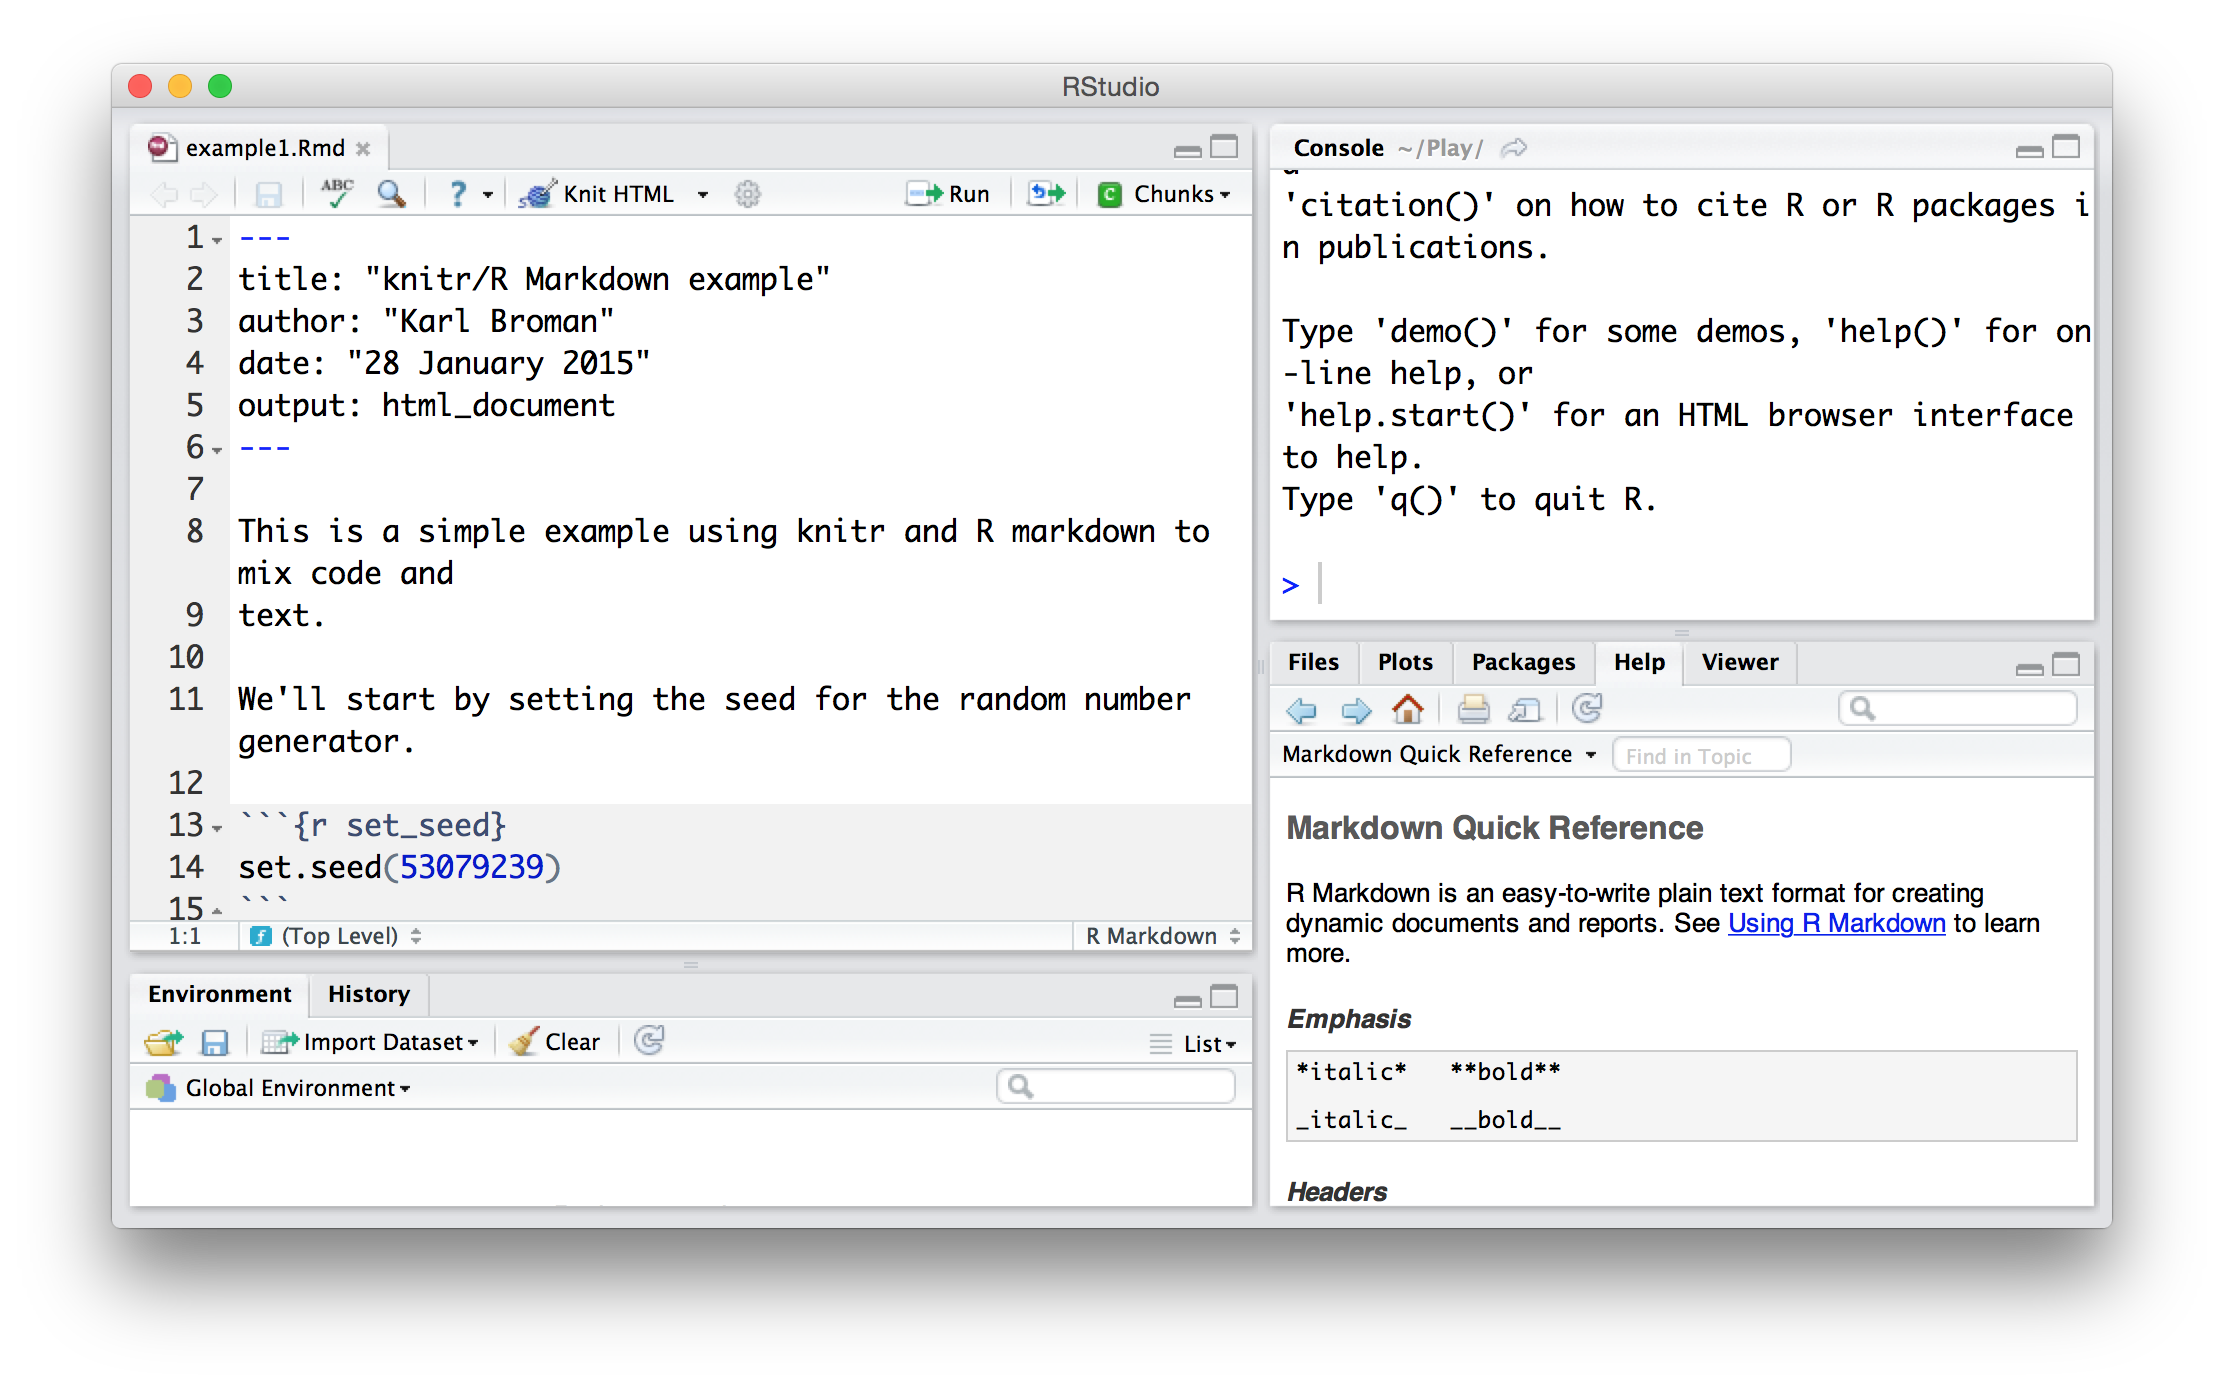
\includegraphics[width=\textwidth]{Figs/rstudio_knitr.png}}

\note{The easiest way to convert an R Markdown file to html is with R
  Studio.

  Open the R Markdown file in R Studio and click the ``Knit HTML''
  button (with the ball of yarn and knitting needle).

  Note the little ``MD'' button next to that. Click that, and you'll
  get the ``Markdown Quick Reference.''

  What actually happens: The {\tt knit} function in the knitr package
  processes all of the code chunks and in-line code and creates a
  Markdown file and possibly a bunch of figure files.

  Then, the {\tt markdownToHTML} function in the markdown package converts the
  Markdown file to an HTML file, with embedded figures.

  RStudio is especially useful when you're first learning R Markdown
  and knitr, as it's easy to create and view the corresponding html
  file, and you have access to that Markdown Quick Reference.
}

\end{frame}


\begin{frame}[fragile]{R Markdown $\rightarrow$ html, in \href{http://www.r-project.org}{R}}

\vspace{18pt}

\begin{lstlisting}
> library(knitr)
> knit("knitr_example.Rmd")
> library(markdown)
> markdownToHTML("knitr_example.md", "knitr_example.html")
\end{lstlisting}

\bigskip

\begin{lstlisting}
> library(knitr)
> knit2html("knitr_example.Rmd")
\end{lstlisting}


\note{When you click the ``Knit HTML'' button in RStudio, it just runs
  some R code for you (and then opens the result in a preview window).

  But you can do the same thing directly, in R.
}
\end{frame}

\begin{frame}[fragile]{R Markdown $\rightarrow$ html,
    \href{http://www.gnu.org/software/make}{GNU make}}

\vspace{24pt}

\begin{lstlisting}
knitr_example.html: knitr_example.Rmd
  R -e 'library(knitr);knit2html("knitr_example.Rmd")'
\end{lstlisting}

\note{I prefer to do this from the command-line, using a Makefile.
  Then it's more obvious what's happening.
}
\end{frame}



\begin{frame}{Reproducible knitr documents}

\vspace{6pt}

\bi
\itemsep8pt
\item Don't use absolute paths like {\tt \vhilit
  {\textasciitilde}/Data/blah.csv}
\item Keep all of the code and data in one directory (and its
  subdirectories)
\item If you {\vhilit must} use absolute paths, define the various directories
  with variables at the top of your document.
\item Use {\tt R --vanilla} or perhaps \\
{\tt \scriptsize R --no-save --no-restore --no-init-file --no-site-file}
\item Use GNU make to document the construction of the final product
   (tell future users what to do)
\item Include a final chunk with {\tt devtools::session\_info()}
\item For simulations, use {\tt set.seed} in your first
   chunk.
\ei

\note{That you've used knitr doesn't mean the work is really {\nvhilit
    reproducible}.  The source and data need to be available to
  others, they need to know what packages were used and how to compile it,
  and then they need to be able to compile it on their system.

  The complicated alternative to {\tt R --vanilla} is if you want to
  still load {\tt {\textasciitilde}/.Renviron}, for example, to define
  {\tt R\_LIBS}.

  If you use {\tt set.seed} at the top of the document, it should be that
  the random aspects will give exactly the same results.
  I'll use \\ {\tt runif(1, 0, 10{\textasciicircum}8)} and then paste that big number
  within {\tt set.seed()}.

  Two anecdotes: The github repository for the Reproducible Research
  with R and R Studio book uses some absolute paths that basically
  make it not reproducible.

  Earn et al. (2014) Proc Roy Soc B 281(1778):20132570 has a really
  nice supplement, written with knitr. But it says, ``The source code
  is available upon request.'' It's not {\nvhilit really}
  reproducible, then.
}
\end{frame}



\begin{frame}[fragile]{Controlling figures}

\vspace{6pt}

\begin{lstlisting}
```{r test_figure, dev.args=list(pointsize=18)}
x <- rnorm(100)
y <- 2*x + rnorm(100)
plot(x,y)
```
\end{lstlisting}

\vfill

{\small
\bi
\itemsep8pt
\item The default is for knitr/R Markdown is to use the {\tt png()}
  graphics device.
\item Use another graphics device with the chunk option {\tt dev}.
\item Pass arguments to the graphics device via the chunk
  option {\tt dev.args}.
\ei
}

\note{Graphics in knitr are super easy. For the most part, you don't
  have to do anything! If a code chunk produces a figure, it will be
  inserted.

  But depending on the type of figure, you might want to try different
  graphics devices. And sometimes you want to pass arguments to the
  graphics device.

  Yesterday (6 Feb 2014), to change the size of axis
  labels, you couldn't just use the pointsize device argument; you'd also
  need to use something like {\tt par(cex.lab=1.5)}. But I posted a
  question about it on StackOverflow, and Yihui Xie responded and then
  immediately fixed the problem. I used a bit of twitter in there too,
  to get his attention.

  To download and install the development version of knitr, you can
  use the {\tt install\_github} function in Hadley Wickham's devtools
  package. Use {\tt install.packages("devtools")} if you don't already
  have it installed.  Then {\tt library(devtools)} and
  {\tt install\_github("yihui/knitr")}.
}
\end{frame}


\begin{frame}[fragile]{Tables}

\vspace{24pt}

\begin{lstlisting}
```{r kable, results="asis"}
x <- rnorm(100)
y <- 2*x + rnorm(100)
out <- lm(y ~ x)
kable(summary(out)$coef, format="html",
      digits=2)
```
\end{lstlisting}

\vspace{12pt}

\begin{lstlisting}
```{r xtable, results="asis"}
library(xtable)
tab <- xtable(coef_tab, digits=c(0, 2, 2, 1, 3))
print(tab, type="html")
```
\end{lstlisting}


\note{Two ways to make tables with R Markdown: the {\tt kable}
  function in the knitr package, and the {\tt xtable} function in the
  xtable package.

  {\tt kable} is simpler, but has fewer options.

  {\tt xtable} gives you more complete control.
}
\end{frame}



\begin{frame}[c]{Important principles}

\centering
Modify your desires to match the defaults.

\vspace{36pt}

Focus your compulsive behavior on things that matter.

\note{Focus on the text and the figures before worrying too much about
  fine details of how they appear on the page.

  And consider which is more important: a manuscript, web page, blog,
  grant, course slides, course handout, report to collaborator,
  scientific poster.

  You can spend a ton of time trying to get things to look just
  right. Ideally, you spend that time trying to construct a general
  solution.  Or you can modify your desires to more closely match what
  you get without any effort.
}
\end{frame}



\end{document}
